\documentclass[11pt]{article}
\usepackage[T1]{fontenc}
\usepackage[margin=1.2in,top=0.6in,bottom=0.6in]{geometry}
\usepackage[bookmarks,colorlinks=true,linkcolor=blue,urlcolor=blue]{hyperref}
\usepackage{url}
\usepackage{tabularx}
\usepackage{graphicx}
\usepackage{placeins}
\usepackage{paralist}
\usepackage{makecell}
\usepackage{colortbl}
\usepackage{gensymb}
\usepackage{textcomp}
%\usepackage[osf]{libertine}
\usepackage{zi4}
\usepackage{float}
\usepackage[libertine,cmbraces]{newtxmath}

\usepackage{draftwatermark}


% table lines
\newcommand{\thinhline}{\Xhline{1\arrayrulewidth}}
\newcommand{\thickhline}{\Xhline{2.5\arrayrulewidth}}
\newcommand{\rtm}{\textsuperscript{\textregistered\space}}

\begin{document}

\title{AKL-PT2 6 GHz Passive Probe Operator Manual}
\author{Antikernel Labs}
\date{\today}

\maketitle
\thispagestyle{empty}

\pagebreak

\tableofcontents

\pagebreak

\section{Overview}

\subsection{Manufacturer}
Antikernel Labs \\
PO Box 4665 \\
10355 NE Valley Rd \\
Rollingbay, WA 98061-0665 \\
\href{https://www.antikernel.net/}{https://www.antikernel.net/} \\
\href{mailto:sales@antikernel.net}{sales@antikernel.net} \\

\subsection{Warranty}

Antikernel Labs warrants this probe to meet published specifications during ordinary laboratory use and operation for a
period of one (1) year from date of shipment and will repair or replace, at its sole option, any defective product.
This warranty covers manufacturing and assembly defects only. Damage caused by negligence, misuse, accident,
alterations, or exceeding published operating limits is specifically not covered. The solder terminals at the probe tip
are consumable and are expected to degrade over time from repeated soldering and desoldering; damage from ordinary wear
and tear is not covered.

Antikernel Labs's maximum liability under this warranty is limited to the replacement value of the probe. Antikernel
Labs will not be liable for any direct, indirect, special, exemplary, or consequential damages (including, but not
limited to, procurement of substitute goods or services, loss of use, data, or profits; or business interruption)
arising in any way out of the use of this probe, even if advised of the possibility of such damage.

\subsection{Open Hardware}

The most up-to-date design files for this probe may be found on GitHub under the 3-clause BSD license, including:

\begin{itemize}
\item KiCAD schematic
\item KiCAD board layout
\item Fabrication notes including stackup and impedance
\item Sonnet field solver models
\end{itemize}

The current location of design files as of this writing is:
\url{https://www.github.com/azonenberg/starshipraider/}.

\subsection{Testing Note}

All AKL-PT2 probes (unless sold under student/hobbyist discount pricing) are soldered to a test fixture during
the manufacturing process using lead-free SAC305 solder in order to verify that they meet all published specifications.
Excess solder and flux is removed prior to shipment, however a small amount of tinning residue remaining on the
castellations is normal.

\pagebreak
\subsection{Sponsors}

Development and prototyping of this probe was made possible by support from
\href{https://www.symbioticeda.com/}{Symbiotic EDA}.


\includegraphics[height=2cm]{symbiotic-logo.png}

\subsubsection{Disclaimer}

Antikernel Labs has terminated its relationship with Symbiotic EDA. The above acknowledgement is required by contract to
remain in the manual and on all probes manufactured prior to April 2023 and should not be construed in any way to imply
endorsement of Symbiotic EDA by Antikernel Labs.

\pagebreak
\section{Safety Information}

To avoid personal injury, damage to the probe, or damage to the attached instrument, it is important to understand and
follow the warnings and specification limits in this document.

\begin{itemize}
\item Only personnel familiar with the safe use and operation of electronic test equipment should use this probe.
\item Do not connect the ground terminal of this probe to any voltage other than earth ground.
\item Do not exceed operating limits in the specifications section of this document.
\item Do not over-tighten the SMA connector. Antikernel Labs recommends using a properly calibrated torque wrench to
torque the connection to 5 lbf-in (0.57 Nm) while holding the connector body across the flats with a wrench. Do not
apply torque without securely holding the connector body.
\item The coverlay on this probe is \emph{not} rated for insulation against hazardous voltages, and conductive elements
are exposed at the tip and connector. Do not use this probe on any circuits which may contain voltages exceeding 30
Vrms, or the touch-safe voltage limit in your organization's standard operating procedures if this is lower.
\item Do not operate in damp or wet conditions, or under temperature/humidity extremes in which condensation is
likely.
\item Do not operate this probe in a flammable or explosive atmosphere.
\item Wear eye protection and ensure good ventilation when soldering.
\item The SMA connector center terminal is made from beryllium copper (BeCu) alloy. While exposure to beryllium is
expected to be insignificant during ordinary use of this product as the BeCu is in solid form and covered by gold
plating, hazardous dust could potentially be generated if the contact material is ground or abraded.

CA PROP 65 WARNING: This product can expose you to beryllium, which is known to the State of California to cause cancer.
\end{itemize}

\pagebreak
\section{Theory of Operation}

Tha AKL-PT2 probe is a \emph{transmission line probe} and works very differently from high-impedance passive or active
probes many engineers are familiar with. It is intended primarily for probing relatively low impedance ($50 \Omega$
range), high bandwidth digital signals, which ordinarily require expensive active probes to properly examine.

\begin{figure}[h]
\centering
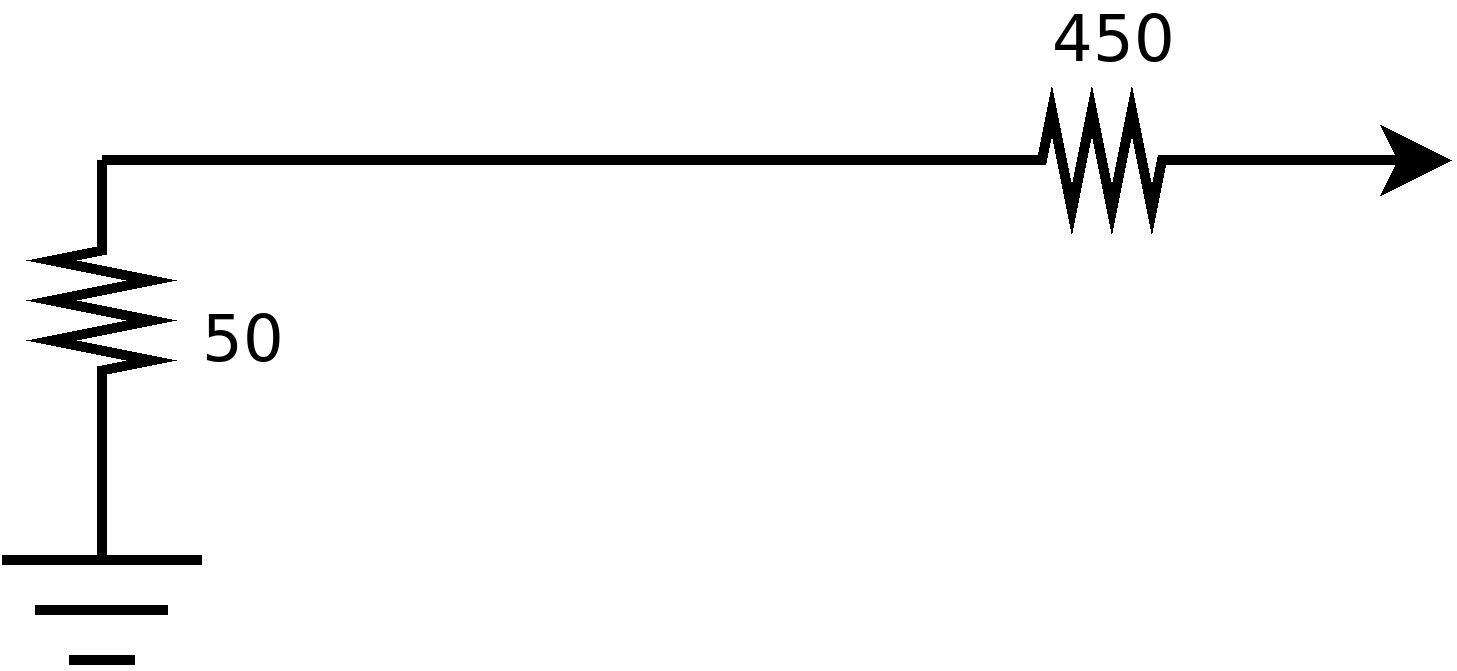
\includegraphics[height=4cm]{schematic.png}
\caption{Simplified probe schematic}
\label{schematic}
\end{figure}

The signal is split off from the DUT at the point of contact and travels through the probe castellations, then passes
through a precision resistor array. This array is a series string of several resistors of different values summing to
450 $\Omega$, carefully selected to cancel out frequency-dependent effects from L/C parasitics and ensure maximal
flatness across the operating frequency range.

The signal then travels on 50 $\Omega$ transmission line through a low-loss coplanar waveguide, SMA connector, and
coaxial cable to the oscilloscope, which terminates the signal with 50 $\Omega$ to ground. The tip resistor and
termination form a 10:1 voltage divider, so the oscilloscope sees the incident signal attenuated by a factor of 10 (-20
dB). \emph{Note that a 50 $\Omega$ termination at the instrument is required. This probe cannot be used with lower-cost
oscilloscopes that only have 1M $\Omega$ terminations.}

The tip resistor and scope-side termination in series present a total loading of 500 $\Omega$ on the DUT. While this is
a significantly lower DC impedance than conventional probes, the resistive input stage has extremely flat frequency
characteristics with much less capacitance than conventional passive probes. This means that the impedance of the probe
remains comparatively constant across the entire operating range, rather than greatly decreasing at higher frequencies.

\pagebreak

\section{Usage Instructions}

Proper soldering and desoldering technique is crucial to getting the best performance and lifetime from your probe.

\subsection{Probe Coupling}

Transmission line probes such as the AKL-PT2 have significantly higher DC loading than a standard $10M\Omega$ passive
probe, and may interact poorly with pull-up/pull-down resistors or level shifters with automatic direction sensing.
Consider AC coupling (using an industry standard SMA inner DC block between the probe and coaxial cable), or use of a
different type of probe for these applications.

\subsection{Test Point Design}

The probe tip is designed to mate with a signal and ground contact on the DUT at 1.0 mm spacing. The suggested test
point layout is shown in Fig. \ref{footprint}. A 1.0 mm long aperture as shown in the diagram is preferable if space
permits, but this may be reduced to 0.5 mm in space-constrained applications. The diagonal trace shows one potential
layout of the signal approaching the test point; arbitrary routing above or below the soldermask aperture is acceptable
as long as the trace is straight within the aperture.

\begin{figure}[h]
\centering
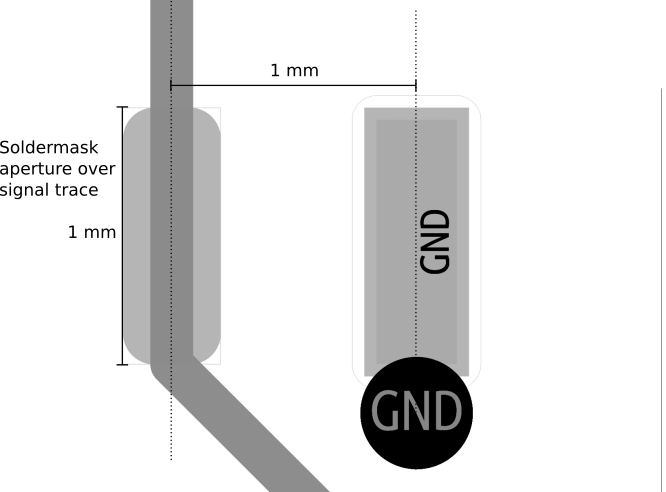
\includegraphics[width=10cm]{footprint.png}
\caption{Suggested test point layout (probe entering from bottom)}
\label{footprint}
\end{figure}

Avoid placing test points in confined spaces between components or in other difficult-to-reach locations. The tip of
the probe is nominally 3.0 mm wide so at least 1.5 mm of clearance to either side of the signal/ground contacts is
required for the tip to fit while providing room for tolerances of PCB edge routing. Additional space beyond this will
likely be needed for effective soldering.

Consider the relative orientation of the signal and ground contacts on the probe when designing test points. If the
probe is oriented with the SMA at the left and the tip at the right, the upper contact is signal and the lower is
ground.

\subsection{Placing and Securing}

The tip castellations are fragile and can be easily damaged by applying even a small amount of force to the solder
joint. When working with any solder-in probe, it is critical to provide a firm mechanical attachment \emph{before}
soldering the tip. Securing a probe operating at microwave frequencies, such as the AKL-PT2, requires additional care
to avoid degrading the performance of the system.

Antikernel Labs recommends use of removable double-sided tape, such as Scotch\rtm part number MMMR103B tape squares or
3M Command\rtm strips, to secure the probe from the underside. Thick foam/gel tape such as these is preferable to
conventional double-sided tapes based on thin plastic films, since increasing the spacing from probe to DUT reduces
capacitive coupling between surface conductors on the DUT and the ground plane on the underside of the probe. An example
of a properly secured probe is shown in Fig. \ref{secured-tip}.

\begin{figure}[h]
\centering
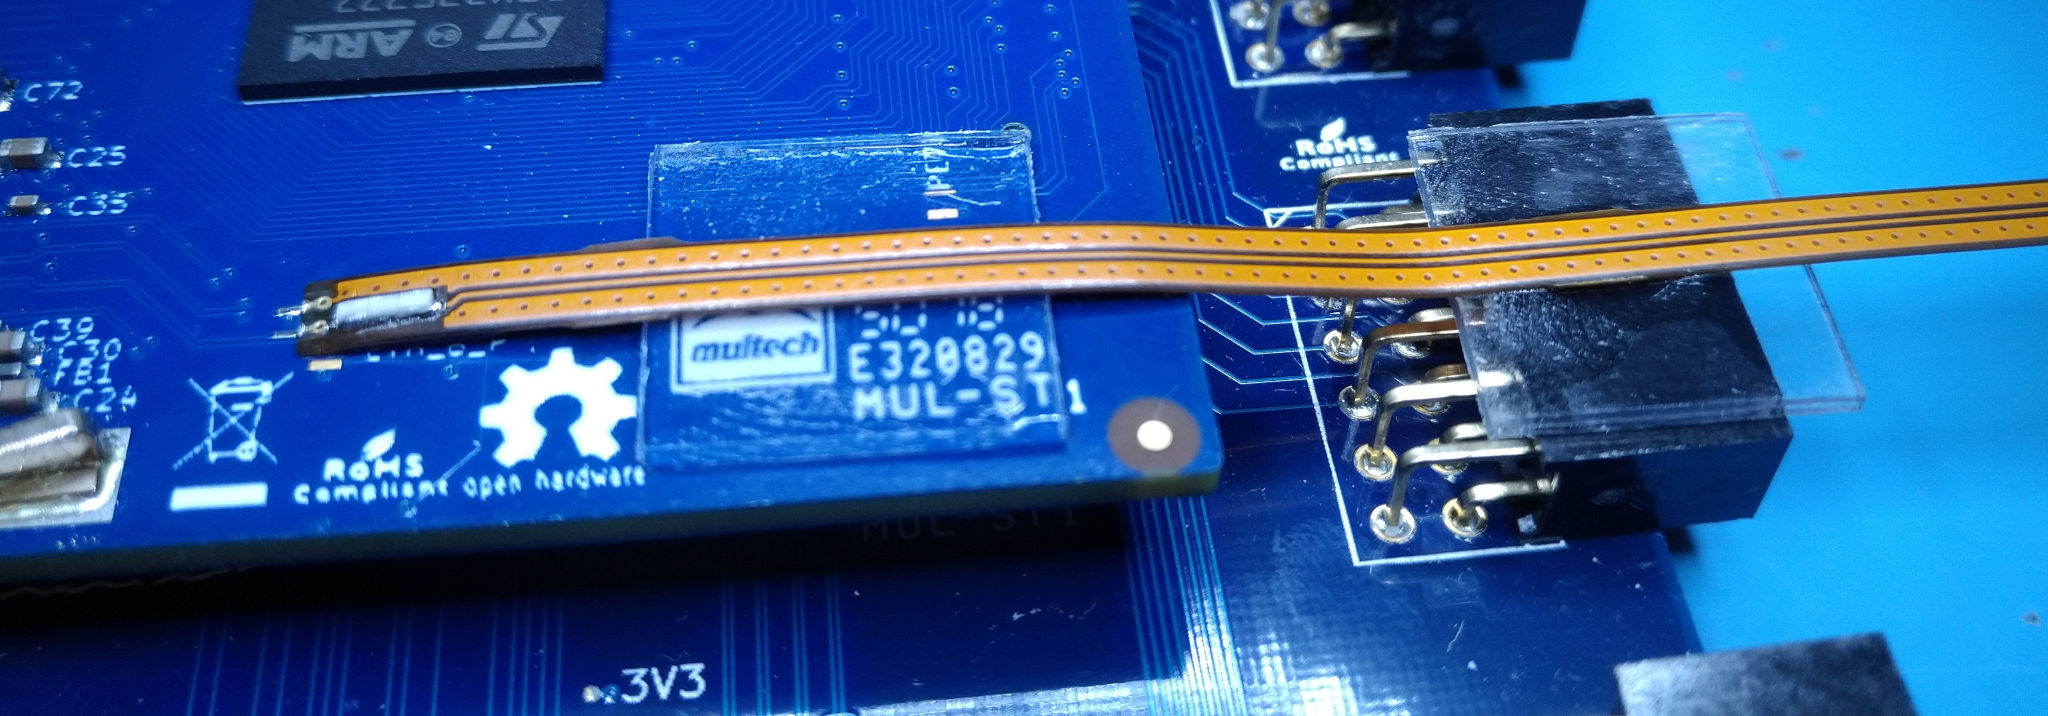
\includegraphics[width=12cm]{secured-tip.jpg}
\caption{AKL-PT2 probe secured to DUT with double-sided adhesive squares}
\label{secured-tip}
\end{figure}

Securing the probe from the bottom side avoids placing any dielectric material over the signal trace, which could cause
the impedance of the probe to shift. If the probe must be secured from the top side, use narrow strips of thin
Kapton\rtm tape to minimize the amount of dielectric added over the signal trace.

To minimize coupling between the probe's ground plane and the DUT, avoid running the probe directly over signal traces
when possible. The tip area is unshielded directly under the resistors and is especially sensitive to EMI. Good results
can often be obtained by securing the probe to the top of an IC package, heatsink, or connector shield, then bending
the end of the probe downward so the castellation contacts the test point at an angle (minimizing the portion of the
probe's length in close proximity to the surface of the DUT). The probe includes a polyimide stiffener under the
resistors and epoxy staking on the top side of the board to reduce the risk of cracking the solder joints, however
deliberate flexing of the probe under or close to the resistors may still cause damage and should be avoided.

The SMA cable attached to the probe should also be secured to prevent applying excessive force to the probe body. Any
method providing adequate mechanical support may be used; an example setup using polyimide tape is shown in Fig.
\ref{cable-secured}.

\begin{figure}[h]
\centering
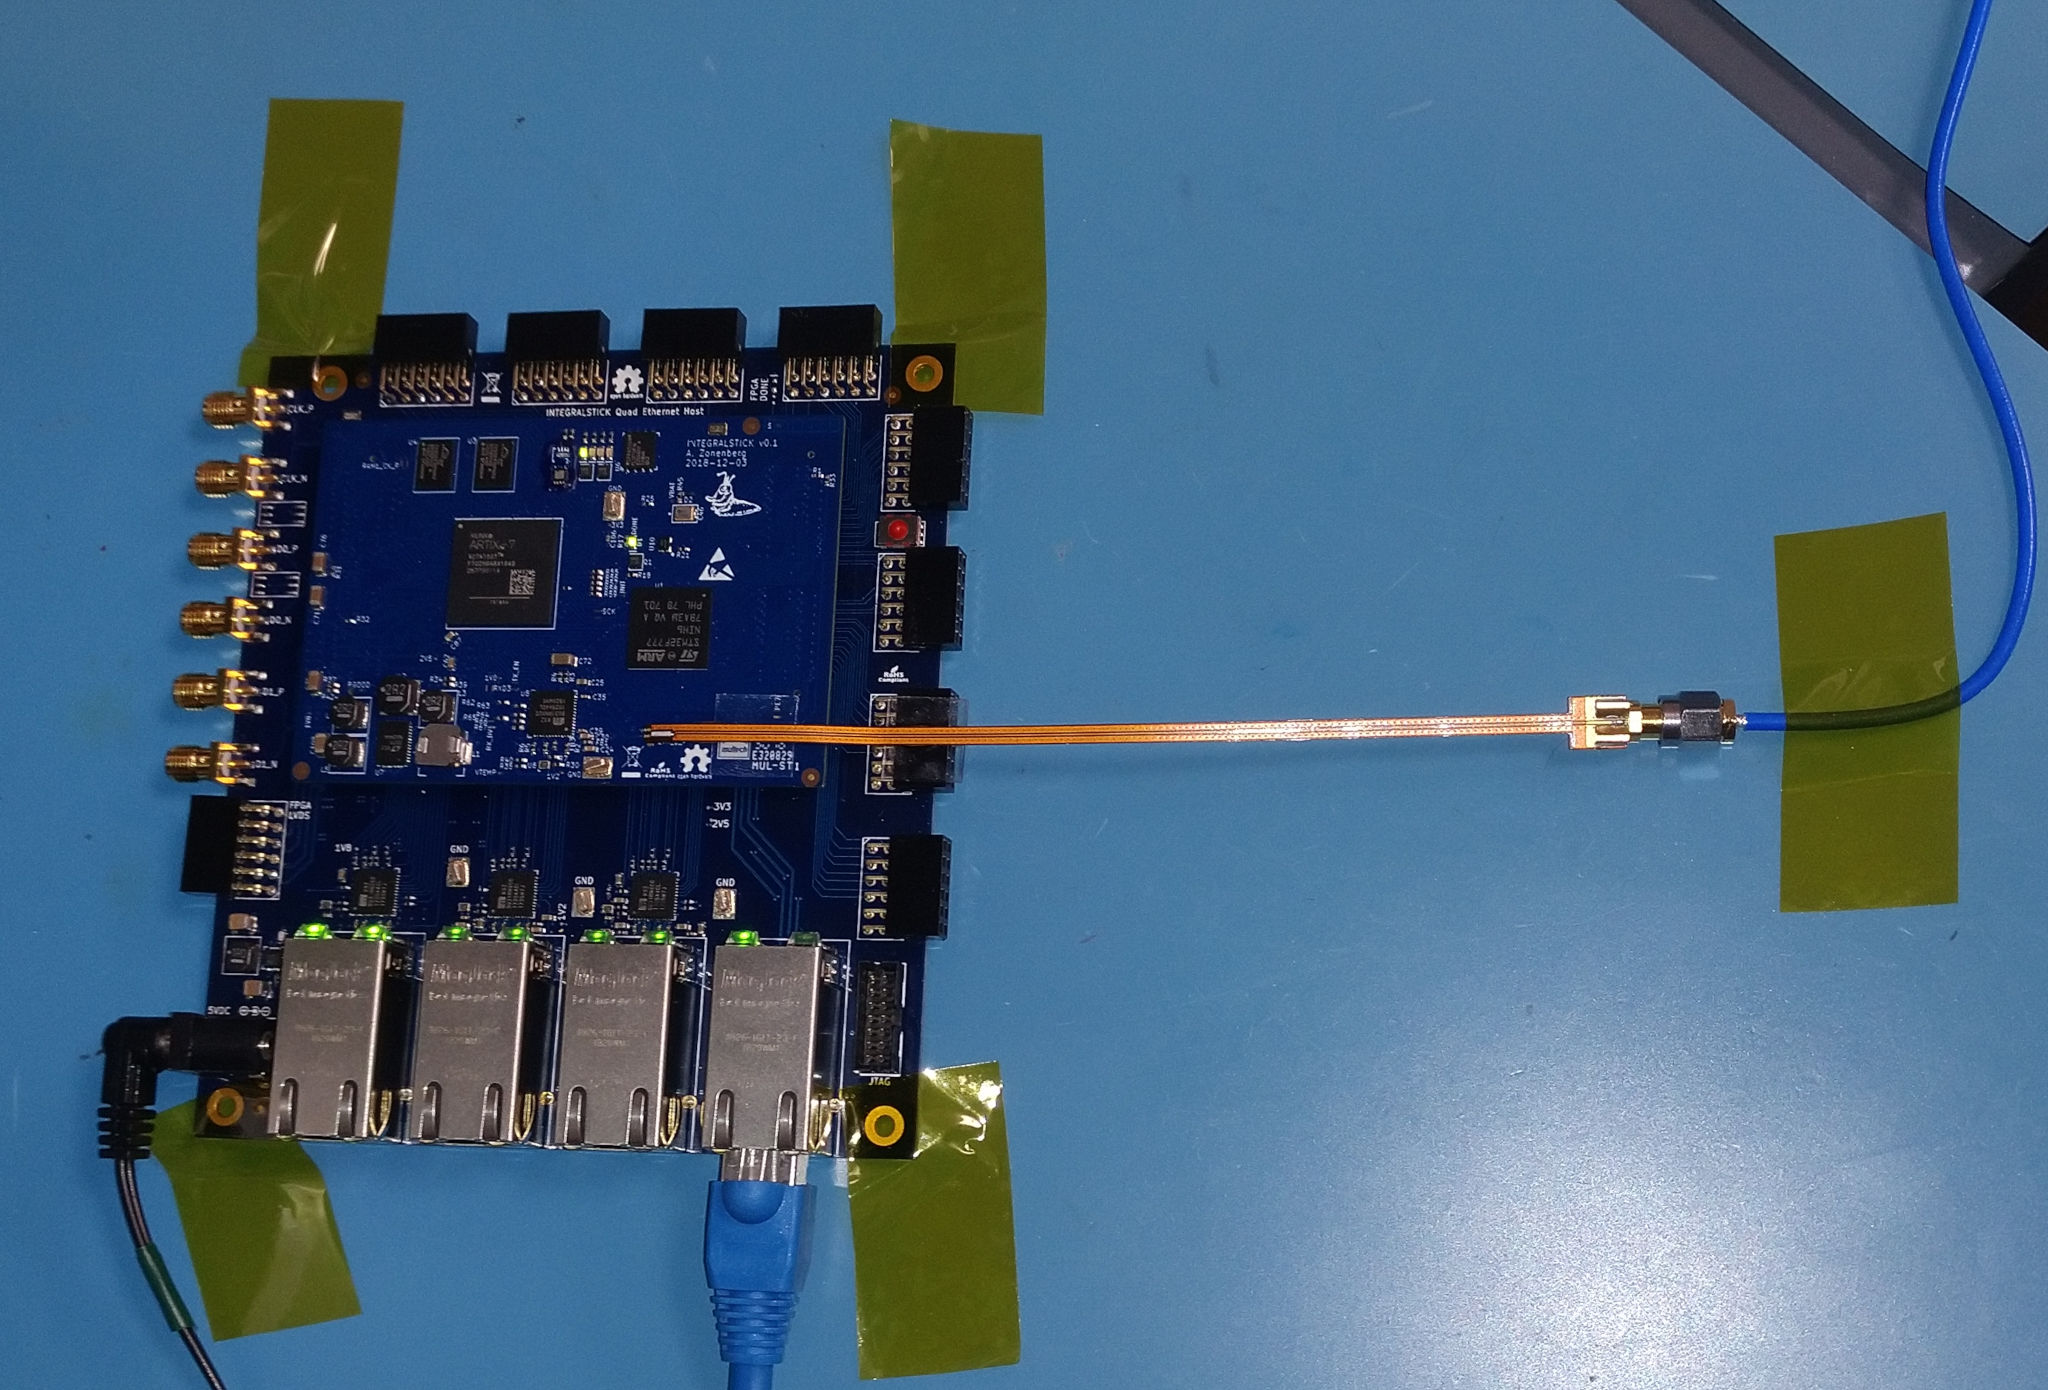
\includegraphics[width=12cm]{cable-secured.jpg}
\caption{Securing cable and DUT to lab bench with polyimide tape}
\label{cable-secured}
\end{figure}

\FloatBarrier

\subsection{Soldering}

Secure the probe body firmly to the DUT, then apply a small amount of flux to the test points. Using a fine point iron
and thin solder wire, solder the signal and ground contacts. Work quickly to avoid overheating the castellations, which
can cause them to delaminate.

For best accuracy and lowest loading, remove flux from the probe tip area after soldering.

\begin{figure}[h]
\centering
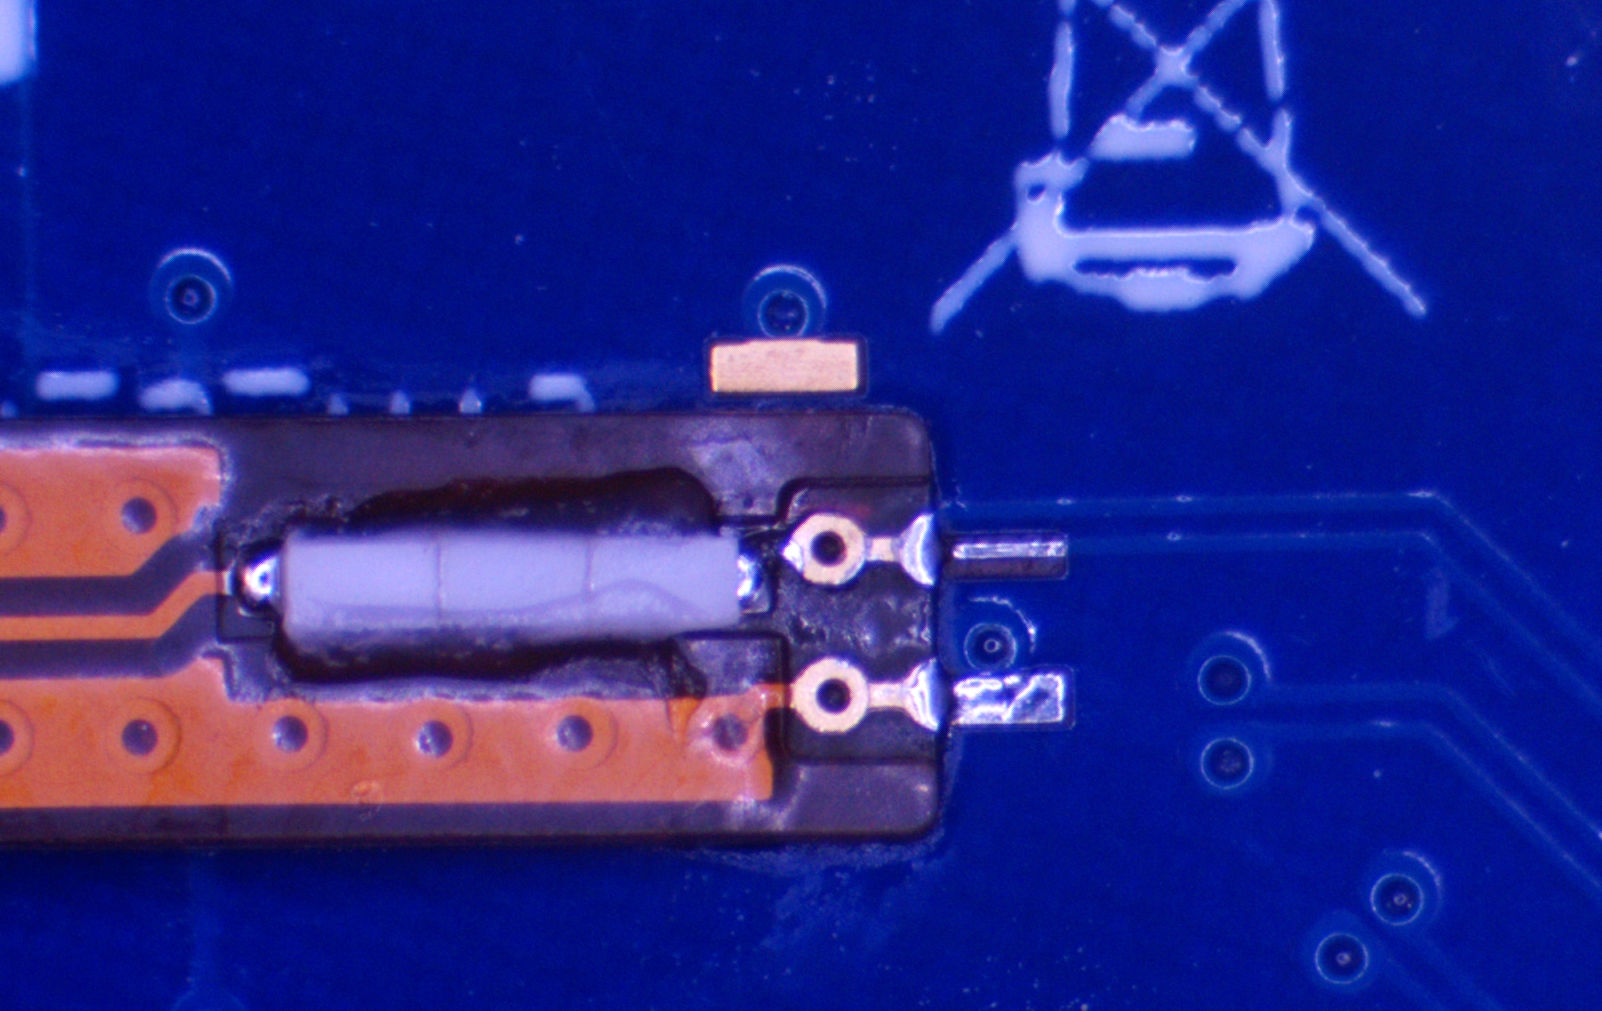
\includegraphics[width=8cm]{tip-on-testpoint.jpg}
\caption{AKL-PT2 tip soldered to test point}
\label{tip-on-testpoint}
\end{figure}
\FloatBarrier

\subsection{Extending the Leads}

If a pre-designed test point is not available, either the signal or ground contact may be extended to fit the board by
means of a short length of 30 AWG (0.255 mm) round copper wire, or flat copper foil wires such as the Circuit Tracks
sold by CircuitMedic\rtm.

For best performance and lowest loading it is crucial to minimize the length of the stub between the test point and the
signal contact; soldering the signal castellation directly to a trace or component lead (as shown in Fig.
\ref{gnd-extend}) is ideal. While excessively long ground leads will degrade performance as well, the probe is far more
tolerant of long ground leads than long signal leads. When extending the ground lead, short and wide wires are
preferable to minimize inductance.

\begin{figure}[h]
\centering
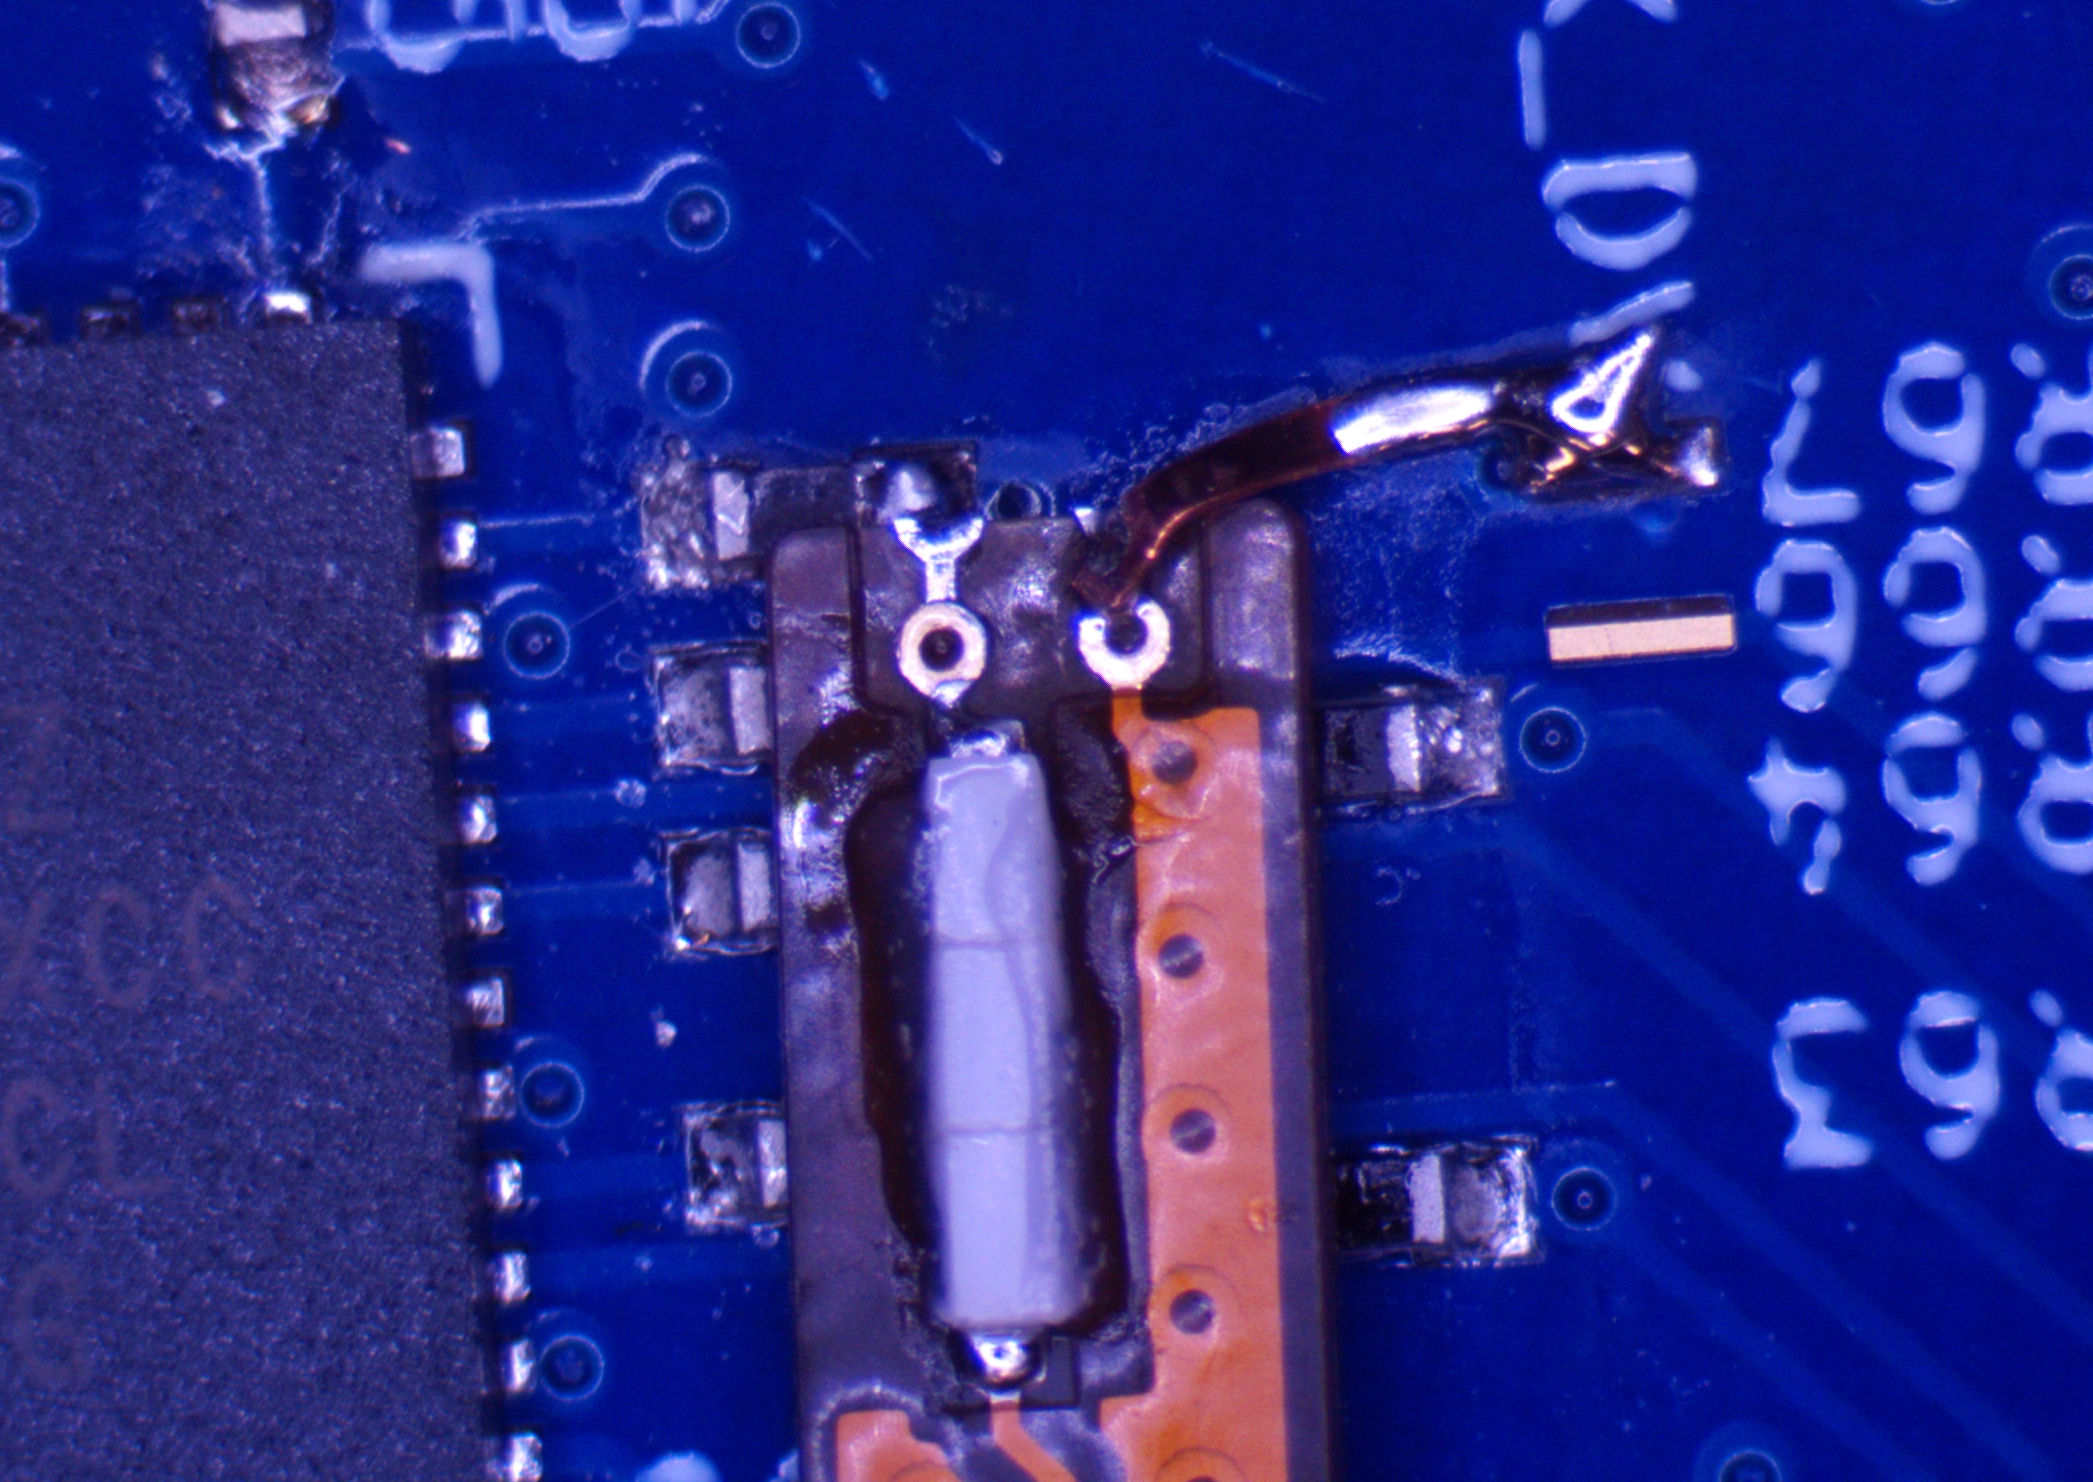
\includegraphics[width=10cm]{gnd-extend.jpg}
\caption{Extending the ground lead with 0.381 mm (15 mil) flat copper wire}
\label{gnd-extend}
\end{figure}

\FloatBarrier

If extending the signal or ground contact is necessary, place the wire horizontally on top of the probe tip and solder
it to the exposed contacts, then bend the wire as needed and solder to the test point.

\subsection{Desoldering}

Use an iron and desoldering braid to remove as much solder from the tip and ground contacts as possible. If the probe
tip does not come free at this point, gently heating with a hot air rework station may be necessary to melt residual
solder on the bottom-side contacts. Once solder on both terminals is visibly melted, gently lift the tip of the probe
away from the board with tweezers and let it cool before removing the tape securing the probe body to the DUT.

If the probe tip was bent into position during the soldering process, be aware that it may be under spring tension and
rapidly stretch back to its natural shape when the solder melts. Use tweezers to support the tip during desoldering to
minimize the chances of sudden tip motion. Allowing the tip to spring away from the board may damage the castellations
if the solder is not fully melted, or fling droplets of molten solder into the air and pose a risk of operator injury.

\subsection{Maintenance, Cleaning, and Storage}

To avoid attracting dust or corroding the tip contacts, when the probe is being stored it is best to remove flux
residue from the tip area. This may be done with isopropyl alcohol and a lint-free swab, or any other industry-standard
flux remover suitable for the flux in question.

The SMA connector on the probe is gaged before shipment to ensure the pin and dielectric position are within tolerance,
however it is good practice to gage the connector periodically to detect any gradual misalignments.

No other maintenance is normally required.

As with any other bare PCB, the probe should be stored flat and protected from mechanical damage.

\FloatBarrier
\subsection{Cables}

The AKL-PT2 must be connected to the host instrument via a $50 \Omega$ coaxial cable rated for at least 7 GHz operation.
Antikernel Labs recommends use of Mini-Circuits \href{https://www.minicircuits.com/pdfs/FL086-24SM+.pdf}{FL086 series}
flexible cable, \href{https://www.minicircuits.com/pdfs/086-24SM+.pdf}{086 series} hand-formable cable, or equivalents.

The cable should be taped to a lab bench or the DUT as shown in Fig. \ref{cable-secured}, or otherwise secured to
prevent transferring any force into the probe.

The probe-side connector is a brass SMA (Amphenol RF 901-10511-3). For best results, this connection should be torqued
to 5 in-lbf (0.57 Nm). Over-tightening may damage the connector. When torquing the connector, hold the connector body
across the flats with a wrench. Do not hold the probe by the PCB as this can put stress on the solder joints or flex
circuitry.

\pagebreak

\section{Mechanical Specifications}

\begin{tabularx}{10cm}{Xrr}
\thickhline
\textbf{Description} & \textbf{Typ} & \textbf{Units} \\
\thickhline
Mass & 2.09 & g\\
\thinhline
Thickness (flex PCB) & 0.3 & mm\\
\thinhline
Length (PCB) & 150.5 & mm\\
\thinhline
Length (total) & 160.3 & mm\\
\thinhline
Width (tip area) & 3.0 & mm\\
\thinhline
Width (connector area) & 8.0 & mm\\
\thickhline
\end{tabularx}

\pagebreak
\section{Electrical Specifications}

Values in this section are typical / limit values. For measured values from a specific probe, please consult your
calibration certificate.

% Assume 0.0015x worst case for resistor base tolerance
% 25 ppm (0.000025x) per degC, -10 / +20C range gives -0.00025 / +0.0005x
% so final range is 0.9975 / 1.005

\subsection{Absolute Maximum Ratings}

Exceeding these limits may result in permanent damage to the probe. Ratings in this section are stress ratings only and
normal operation at these limits is not implied.

\begin{tabularx}{12cm}{lXrl}
\thickhline
\textbf{Parameter} & \textbf{Description} & \textbf{Limit} & \textbf{Units} \\
\thickhline
$T_{amin}$ & Minimum temperature & 0 & $ \degree C$ \\
\thinhline
$T_{amax}$ & Maximum temperature & 95 & $ \degree C$ \\
\thinhline
$I_{max}$ & Maximum sustained current & 15.8 & $ mA $ \\
\thinhline
$V_{maxT}$ & Maximum sustained tip voltage & 7.9 & $ Vrms $ \\
\thinhline
$V_{maxV}$ & Maximum instantaneous tip voltage & 50.0 & $ Vrms $ \\
\thickhline
\end{tabularx}

ENGINEERING NOTE: The sustained current/voltage limits are thermally limited and based on the 50 mW power rating of the
$200 \Omega$ tip resistors. Brief pulses or low duty cycle waveforms whose average power does not exceed these limits
\emph{may} be possible to probe safely with the AKL-PT2 as long as tip voltage does not exceed the instantaneous
voltage limit at any time, however Antikernel Labs has not performed any testing of the probe under pulsed load
conditions. Use of the probe with instantaneous power levels exceeding the thermal limits will void the warranty and
customer assumes all risk of harm to personnel and equipment resulting from such usage.

\subsection{Recommended Operating Conditions}

While the probe will not be damaged by exposure to conditions outside the values in this section (but below the
``Absolute Maximum Ratings" limits), tolerances may be temporarily exceeded.

\begin{tabularx}{12cm}{lXll}
\thickhline
\textbf{Parameter} & \textbf{Description} & \textbf{Limit} & \textbf{Units} \\
\thickhline
$T_{min}$ & Minimum temperature & 15 & \degree C \\
\thinhline
$T_{max}$ & Maximum temperature & 45 & \degree C \\
\thinhline
\thickhline
\end{tabularx}

\subsection{DC Characteristics}

\begin{tabularx}{16cm}{lXrrrr}
\thickhline
\textbf{Parameter} & \textbf{Description} & \textbf{Min} & \textbf{Typ} & \textbf{Max} & \textbf{Units} \\
\thickhline
$G_{dc}$ & Gain across high-Z load* &  & 0.1 &  & V/V \\
\thinhline
$R_{gnd}$ & Resistance from SMA shell to tip ground & 0.15 & 0.35 & 0.55 & $\Omega$ \\
\thinhline
$R_{sig}$ & Resistance from SMA pin to tip contact & 450.20 & 450.39 & 450.60 & $\Omega$ \\
\thinhline
$TCR$ & Temperature coefficient of resistance & & & $\pm 25$ & ppm / \degree C \\
\thickhline
\end{tabularx}

* The tip resistors have $\pm 0.1\%$ accuracy which is significantly better than typical $50 \Omega$ instrument
terminations. DC gain accuracy in actual use is largely dependent on tolerance of the termination at the oscilloscope,
which is typically $\pm 2\%$.

\pagebreak
\subsection{AC Characteristics}

Data in this section is based on characterization in a $50 \Omega$ environment, with cable and fixture effects
de-embedded, unless otherwise stated.

\begin{tabularx}{16cm}{lXrrrr}
\thickhline
\textbf{Parameter} & \textbf{Description} & \textbf{Min} & \textbf{Typ} & \textbf{Max} & \textbf{Units} \\
\thickhline
$S_{11o\_low}$ & $S_{11}$ (open circuit) from DC - 4 GHz & -1.85 & -1.75 & -1.40 & dB \\
\thinhline
$S_{11o}$ & $S_{11}$ (open circuit) from DC - 6 GHz & -2.60 & -1.75 & -1.40 & dB \\
\thinhline
$S_{11\_low}$ & $S_{11}$ across $50\Omega$ from DC - 4 GHz & -33.00 & -22.00 & -14.00 & dB \\
\thinhline
$S_{11\_hi}$ & $S_{11}$ across $50\Omega$ from 4 - 6 GHz & -20.00 & -11.00 & -8.75 & dB \\
\thinhline
$S_{21}$ & $S_{21}$ from DC - 6 GHz & -23.50 & -21.95 & -20.00 & dB \\
\thinhline
$S_{21\_100}$ & $S_{21}$ at 0.1 GHz & -20.50 & -20.45 & -20.40 & dB \\
\thinhline
$S_{21\_500}$ & $S_{21}$ at 0.5 GHz & -21.00 & -20.85 & -20.70 & dB \\
\thinhline
$S_{21\_1000}$ & $S_{21}$ at 1.0 GHz & -21.20 & -21.00 & -20.80 & dB \\
\thinhline
$S_{21\_3000}$ & $S_{21}$ at 3.0 GHz & -22.20 & -21.95 & -21.70 & dB \\
\thinhline
$S_{21\_6000}$ & $S_{21}$ at 6.0 GHz & -23.50 & -23.10 & -22.60 & dB \\
\thinhline
$BW$ & -3 dB bandwidth & 6.00 & 6.50 & & GHz \\
\thinhline
$Rise_{90}$ & Rise time (10-90 \%) & xx & xx & xx & ps \\
\thinhline
$Rise_{80}$ & Rise time (20-80 \%) & xx & xx & xx & ps \\
\thinhline
$Tpd$ & Propagation delay &  & 925 &  & ps \\
\thickhline
\end{tabularx}

\pagebreak
\section{Performance Graphs}

\subsection{Insertion Loss}

\begin{figure}[h!]
\centering
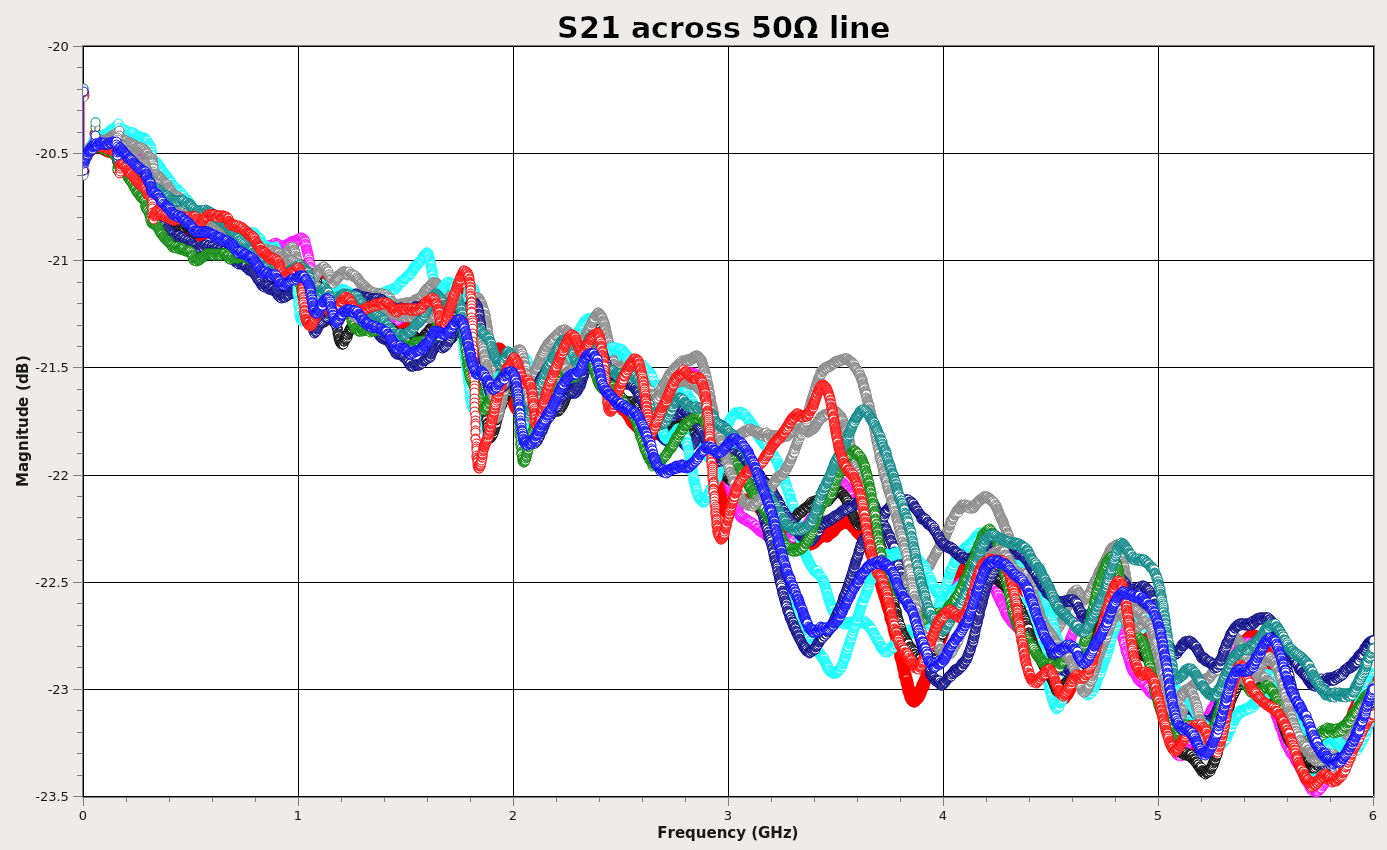
\includegraphics[width=14cm]{s21-variation.png}
\caption{$S_{21}$ range of probes across $50\Omega$ termination}
\label{s21-variation}
\end{figure}

\subsection{Group Delay}

\begin{figure}[h]
\centering
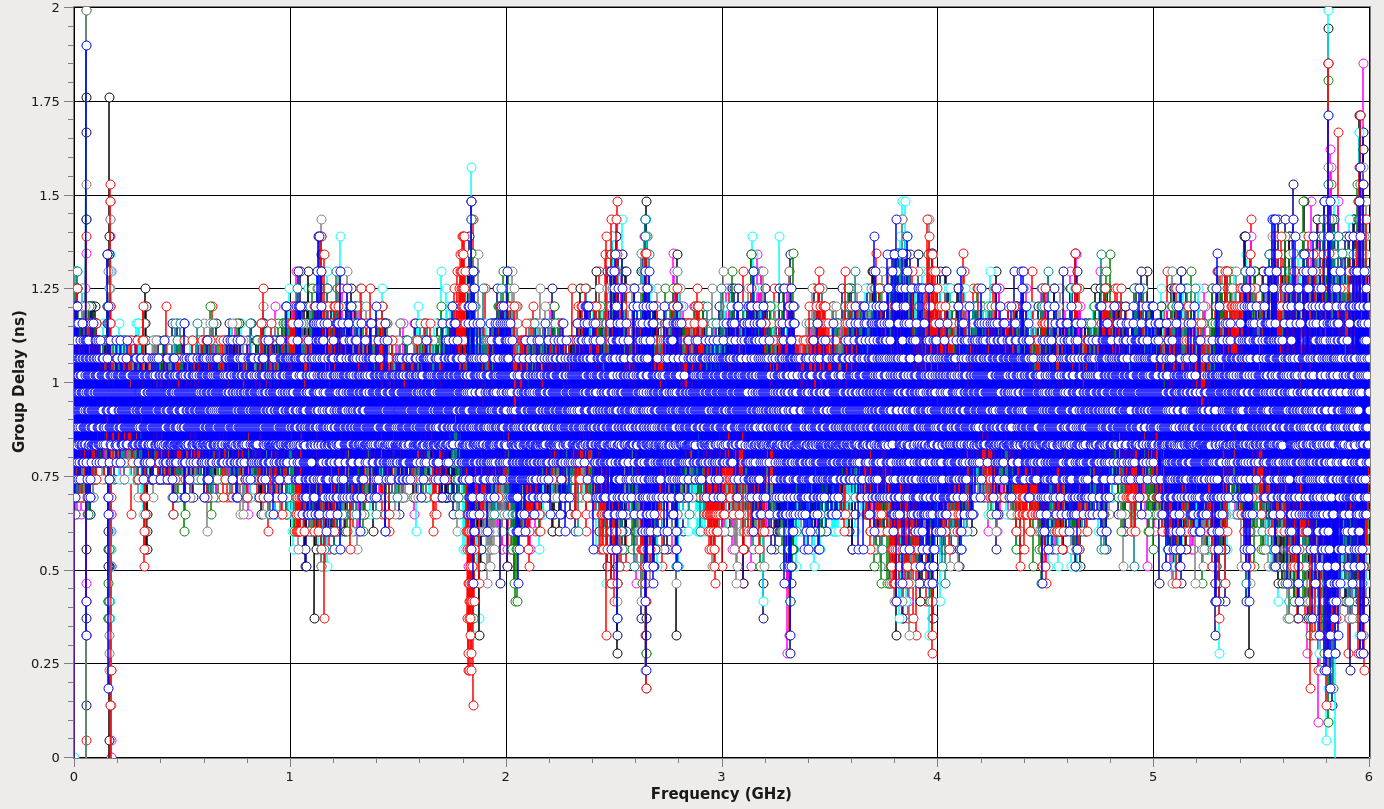
\includegraphics[width=14cm]{groupdelay-variation.png}
\caption{Group delay variation of probes}
\label{typical-groupdelay}
\end{figure}
\FloatBarrier

\pagebreak
\subsection{Return Loss}

\begin{figure}[h!]
\centering
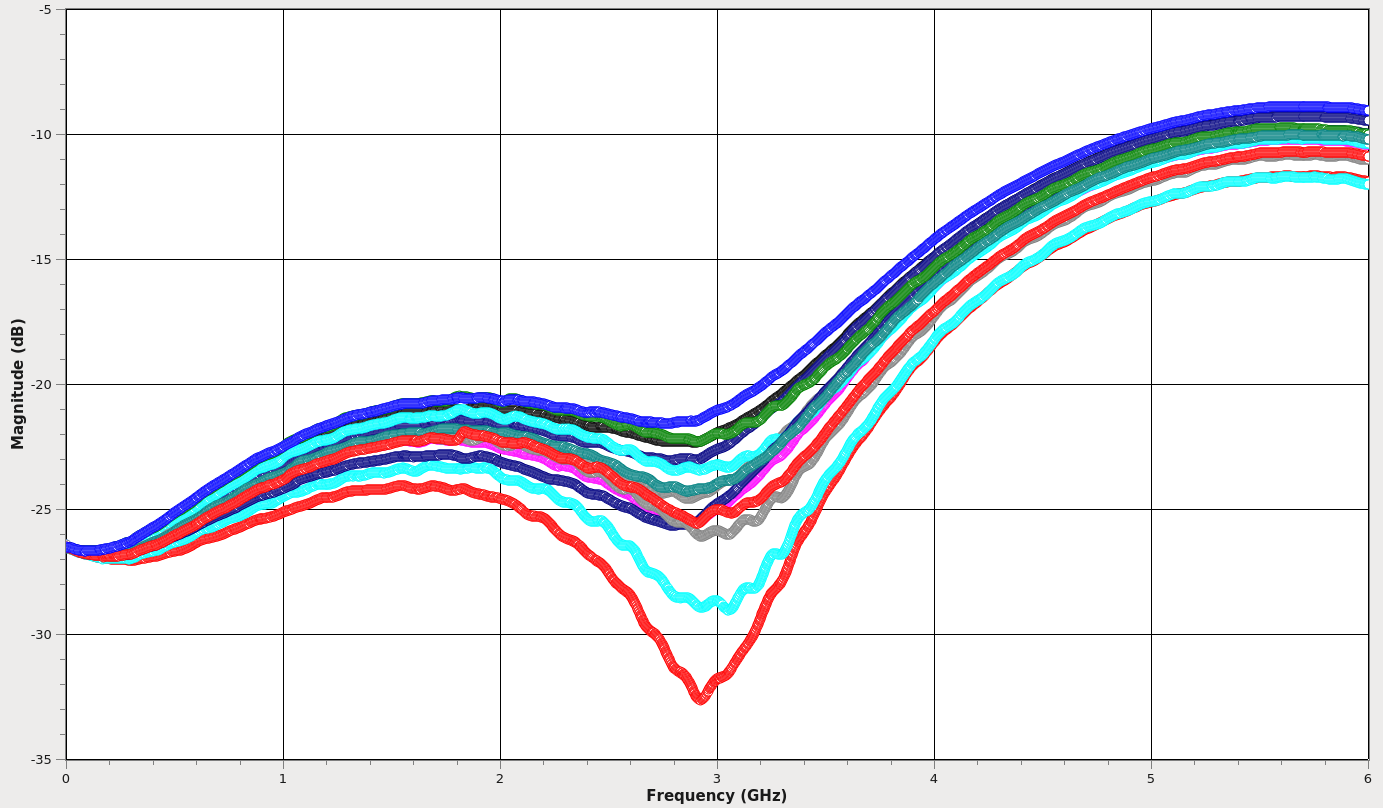
\includegraphics[width=14cm]{s11-variation.png}
\caption{Variation in $S_{11}$ of probes across $50\Omega$ load}
\label{s11-open-variation}
\end{figure}

\begin{figure}[h!]
\centering
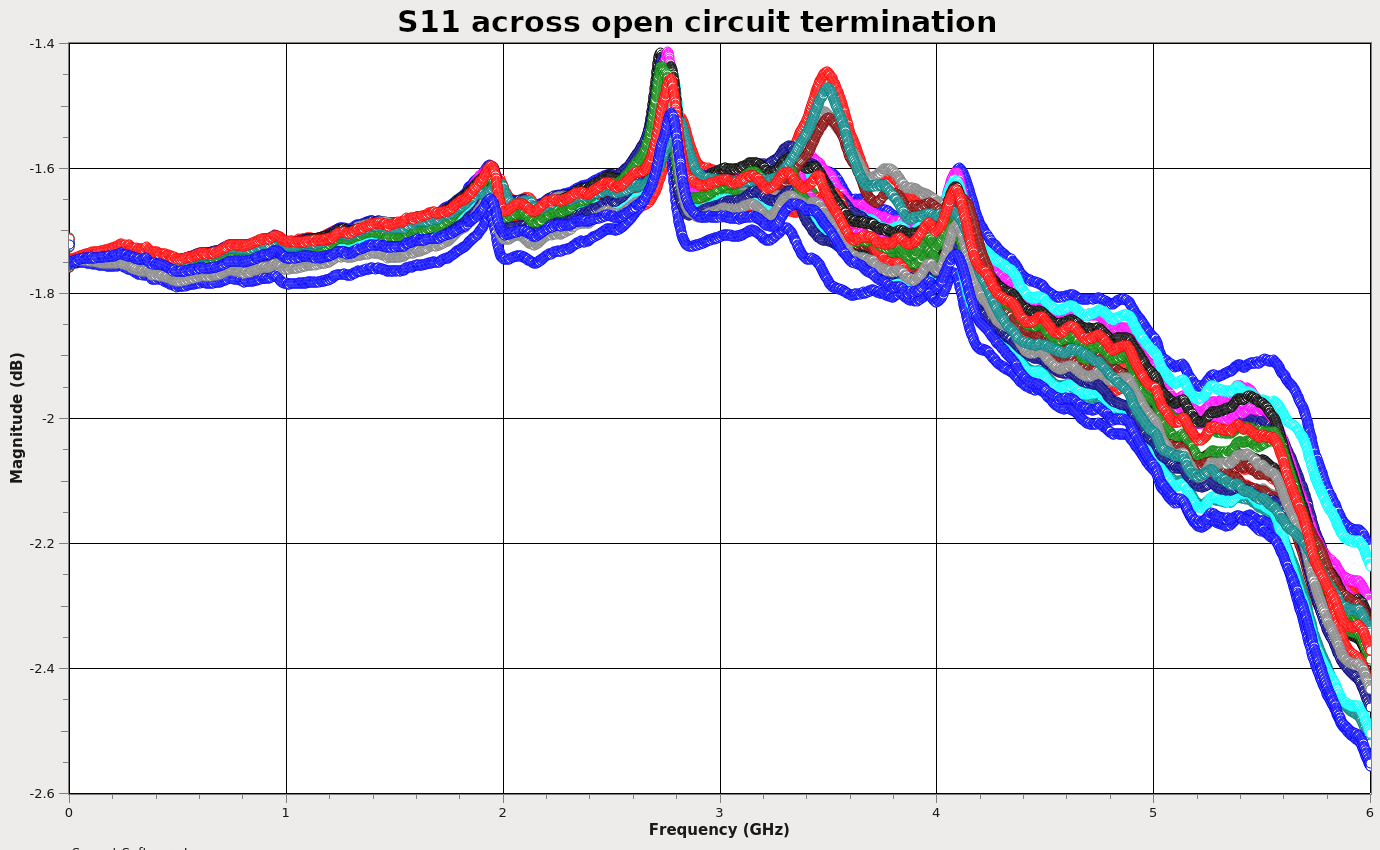
\includegraphics[width=14cm]{s11-open-variation.png}
\caption{Variation in $S_{11}$ of probes across open circuit}
\label{s11-variation}
\end{figure}

\FloatBarrier

\pagebreak
\section{Performance Data}

If you requested full characterization at the time of your order, test measurements are available at
\url{https://www.antikernel.net/downloads/AKL-PT2/caldata/} and searching for your probe's serial number. All
measurements are de-embedded to the SMA connector or probe tip, as applicable.

The following S-parameter data files are provided:
\begin{itemize}
\item cable.s2p - the provided cable (if applicable)
\item probe.s2p - probe soldered across $50 \Omega$ load
\item zin.s1p - probe soldered across an unterminated line for input loading/impedance measurements
\end{itemize}

Touchstone port 1 is connected to the DUT side of the probe and port 2 (if applicable) is connected to the instrument
side.

\end{document}
